\documentclass[../../main.tex]{subfiles}
\usepackage{pgfplots}
\pgfplotsset{compat=1.18}
\begin{document}
\chapter{Intermediate Blocks, Motion Curves, and AZee Templates}
\label{ch:intermediate_blocks}

Creativity in human expression often lies at the intersection of structure and flexibility. In Sign Language, meaning is not just conveyed through individual signs but through the seamless transitions and interactions between them. These transitions, or intermediate blocks, play a crucial role in maintaining the natural flow of communication, ensuring that the message remains clear and expressive.

Generating these intermediate blocks in multi-track representations requires a blend of procedural precision and adaptive techniques. The complexity of Sign Language demands more than linear models; it requires an approach that can reflect the nuances of real-life communication. By integrating the AZee model with multi-track timelines, this chapter explores how we can improve the accuracy and fluidity of synthesized Sign Language.

This chapter focuses on the generation of intermediate blocks within the multi-track representations introduced in chapter~\ref{ch:multi-track}. By utilizing motion templates and carefully interpolating between keyframes, we aim to enhance the naturalness and coherence of Sign Language synthesis, bridging the gap between procedural methods and the dynamic nature of human communication.

In this chapter, section~\ref{ch:intermediate_blocks:related_work} discusses the related work on AZee Templates, Motion Curves, and Motion Templates. Section~\ref{ch:intermediate_blocks:intermediate_block_generation} explores the generation of intermediate blocks, while section~\ref{ch:intermediate_blocks:results} presents the results of this process. Finally, section~\ref{ch:intermediate_blocks:conclusion_and_future_work} concludes the chapter and outlines potential future directions for this research.

\section{Related Work}
\label{ch:intermediate_blocks:related_work}

In this section we will discuss the related work on AZee Templates, Motion Curves, and Motion Templates. 

\subsection{AZee Templates}
\label{ch:intermediate_blocks:related_work:azee_templates}

AZee templates are abstract representations used in sign language synthesis, linking linguistic descriptions with animated motions. For example, an AZee template like \texttt{:info-about(:car,?color)} could match an expression such as \texttt{:info-about(:car,:red)}, where the variable \texttt{color} would be assigned the value \texttt{:red}. This template instructs the avatar to convey information about a car's color, where the specific color (red, in this case) is dynamically inserted based on the template match. This approach allows for the dynamic generation of animations based on linguistic input, enabling avatars to respond to a wide range of queries and commands.

\subsection{Motion Curves}
\label{ch:intermediate_blocks:related_work:motion_curves}

Motion curves, (often refered as function curves or F-curves), have been extensively used in 3D character animation to control the timing and spacing of movements. These curves provide a graphical representation of a parameter's change over time, making them an essential tool in achieving realistic and fluid motion in animations(figure~\ref{fig:fcurves_blender}). Early foundational work by Witkin and Kass~\cite{witkin1988spacetime} introduced spacetime constraints, which used optimization techniques to control motion curves in generating realistic animations under physical constraints. This idea has evolved, and modern techniques now integrate deep learning models with motion curves to enhance control and automate the generation of complex animations.

In the context of Sign Language,~\cite{inproceedings} discuss the use of 3D motion analysis to accurately capture and animate sign language gestures by extracting motion curve parameters from sensors like Microsoft Kinect. These motion curves, which represent the trajectories of movements made during signing, are essential for animating virtual signers in a natural and precise manner. The paper highlights how these curves are mathematically defined, including their type, plane of motion, and velocity, which are then used to recreate realistic sign language animations, enhancing applications like sign language recognition and machine translation.

\begin{figure}
    \centering 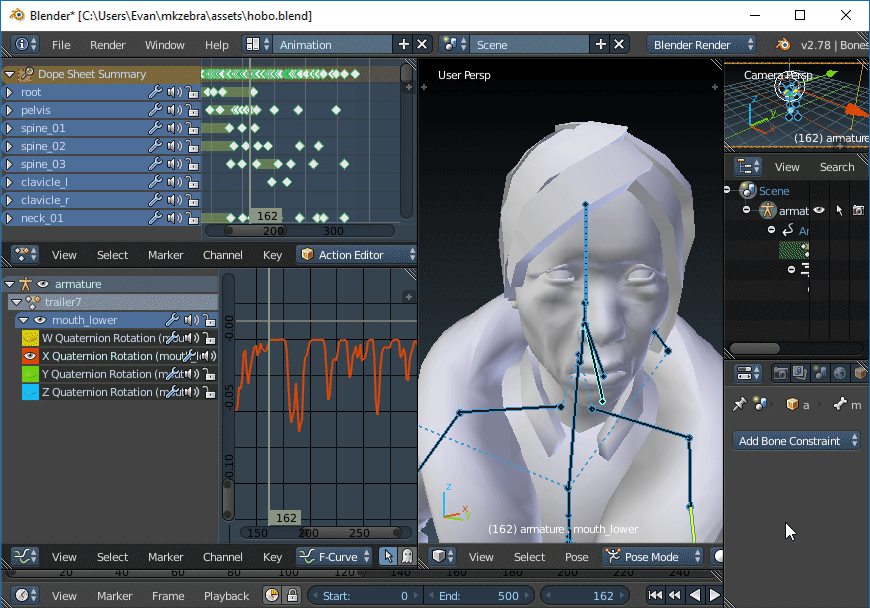
\includegraphics[width = 2.5in]{chapters/intermediate_blocks/images/fcurves_blender.png}
    \caption{F-curves in Blender}
    \label{fig:fcurves_blender}
\end{figure}

In recent research, deep learning methods have been employed to interpret and adapt F-curves for motion inbetweening tasks(figure~\ref{fig:inbetweening_transformers})~\cite{10.1145/3550454.3555454}. However, traditional mathematical optimization techniques are still widely in use(figure~\ref{fig:inbetweening_disney})~\cite{10.1145/3306346.3322938}.

\begin{figure}
    \centering 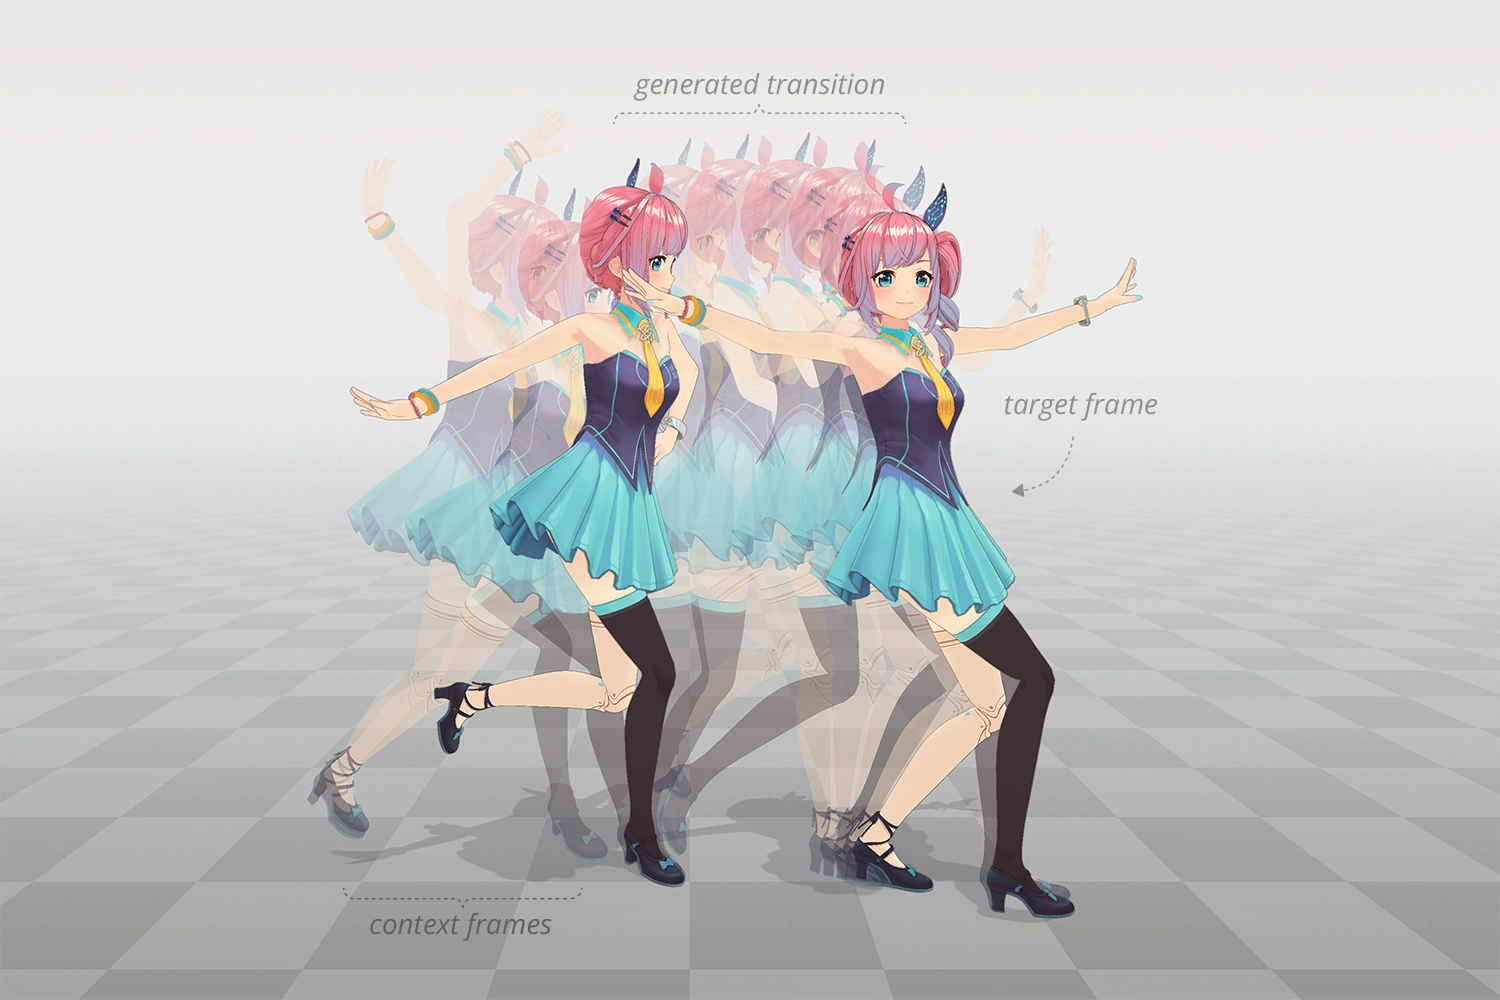
\includegraphics[width = 2.5in]{chapters/intermediate_blocks/images/inbetweening_transformers.jpg}
    \caption{Motion Inbetweening using 2 stage Transformers~\cite{10.1145/3306346.3322938}}
    \label{fig:inbetweening_transformers}
\end{figure}

\begin{figure}
    \centering 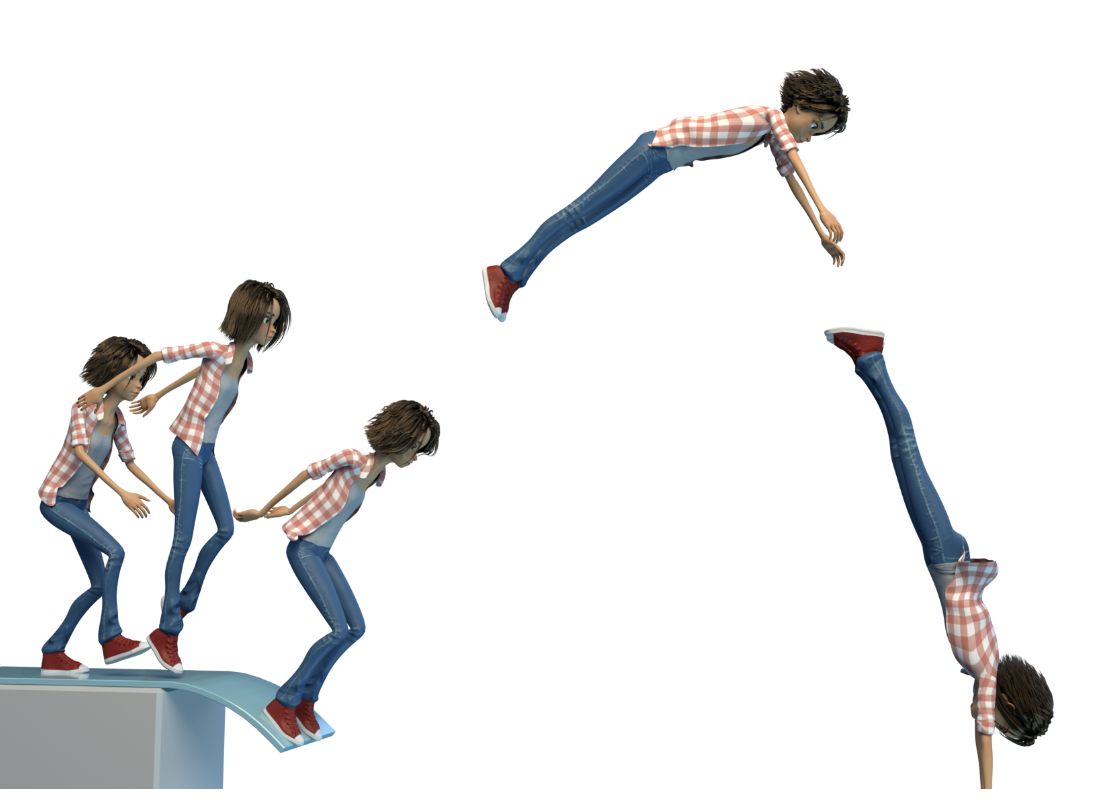
\includegraphics[width = 2.5in]{chapters/intermediate_blocks/images/inbetweening_disney.png}
    \caption{Rig Control using Tangent-Space Optimization}
    \label{fig:inbetweening_disney}
\end{figure}


\subsection{Motion Templates}
\label{ch:intermediate_blocks:related_work:motion_templates}

Motion templates offer a reusable framework for applying pre-defined motion patterns across different characters or scenarios. These templates are essentially built upon motion curves that define the motion's parameters, allowing for efficient replication and adaptation of complex motions. The concept of motion templates has been widely adopted in various fields, from character animation to robotic motion planning. Modern approaches often combine motion templates with machine learning techniques to facilitate the adaptation of these templates to new contexts, such as different character anatomies or environmental conditions.

In the context of character animation, motion templates can be particularly advantageous. The reusable nature of these templates allows for the consistent production of motion across different avatars while ensuring that the nuances of each motion are preserved. A method for controlling avatars using clustered motion segments from a large motion capture database was introduced by~\cite{10.1145/566654.566607}, enabling efficient real-time animation with intuitive user interfaces.

The Paula avatar uses AZee geometric templates that can be applied across various signing scenarios. For example, a rule such as place-prf(proform-vehicle, midssp) allows for the placement of a vehicle proform in the middle of the signing space(figure~\ref{fig:azee_template_example}). This method leverages a consistent geometric system, enabling the natural synthesis of movements without relying on a fixed set of points, which is crucial for capturing the variability and dynamism inherent in sign language. This approach however, generates animations by focusing solely on higher-level linguistic structures rather than low-level positional data.

\begin{figure}
    \centering 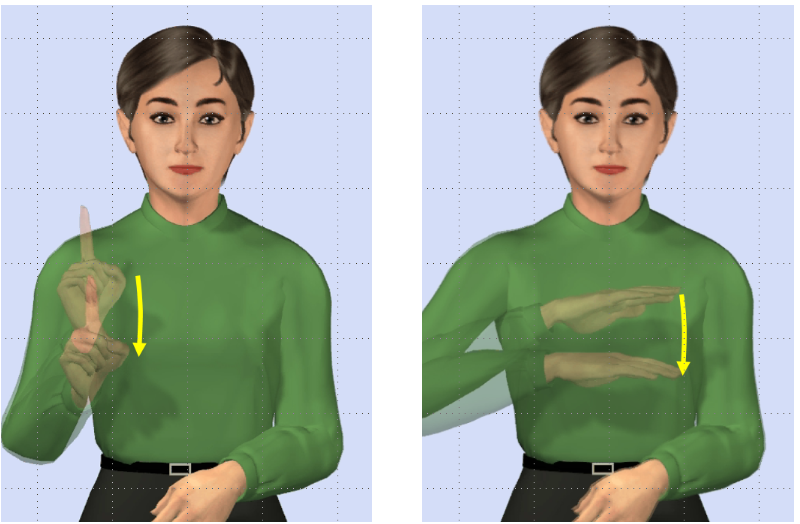
\includegraphics[width = 2.5in]{chapters/intermediate_blocks/images/azee_template_example.png}
    \caption{AZee Templates used by the Paula avatar}
    \label{fig:azee_template_example}
\end{figure}

\section{Intermediate Block Generation}
\label{ch:intermediate_blocks:intermediate_block_generation}

Intermediate blocks are blocks of motion not specified by the AZee model. Building on the concepts of motion curves and templates, intermediate block generation is a process in creating smooth transitions between constrained and pre-animated blocks. Interpolation techniques, such as linear and spline interpolation, can be used to generate intermediate poses or frames that maintain the semantic consistency of the intended sign.

The creation of this intermediate block relies on a template expression check which determines the motion template to be used. 

\subsection{Reusing Motion Templates}
\label{ch:intermediate_blocks:reusing_motion_templates}

Motion templates are pre-defined motion patterns that guide the synthesis of new animations. In the context of AZee driven synthesis, these templates serve as a blueprint for generating intermediate blocks and motion curves. The use of motion templates allows for greater consistency and control over the final animation, as the templates encode expert knowledge about how certain signs should be performed.

These motion templates are based on the template of the AZee rule and can be artistically created or procedurally generated. Figure~\ref{fig:top_down_search_template} shows a top-down search algorithm for selecting the best motion template based on the AZee rule \emph{info-about(cat,cute)}.

\begin{figure}
    \centering 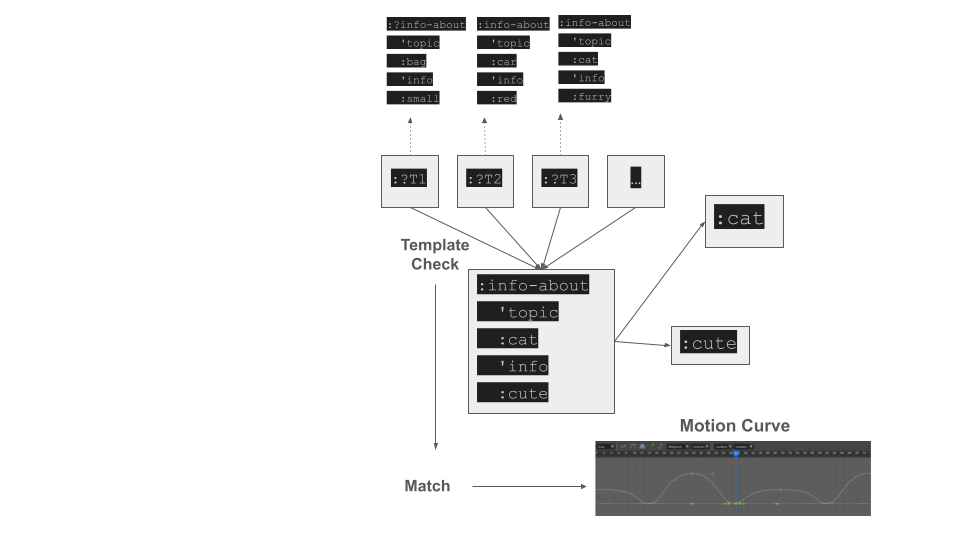
\includegraphics[width = 4in]{chapters/intermediate_blocks/images/top_down_search_template.png}
    \caption{Top-Down Search for Motion Template}
    \label{fig:top_down_search_template}
\end{figure}

The procedurally generated templates can be based on the AZee rule and corresponding motion data. For example, motion curves for the template \texttt{info-about} can be seen in the following figure~\ref{fig:motion_curves_template_procedural}.

\begin{figure}
    \centering 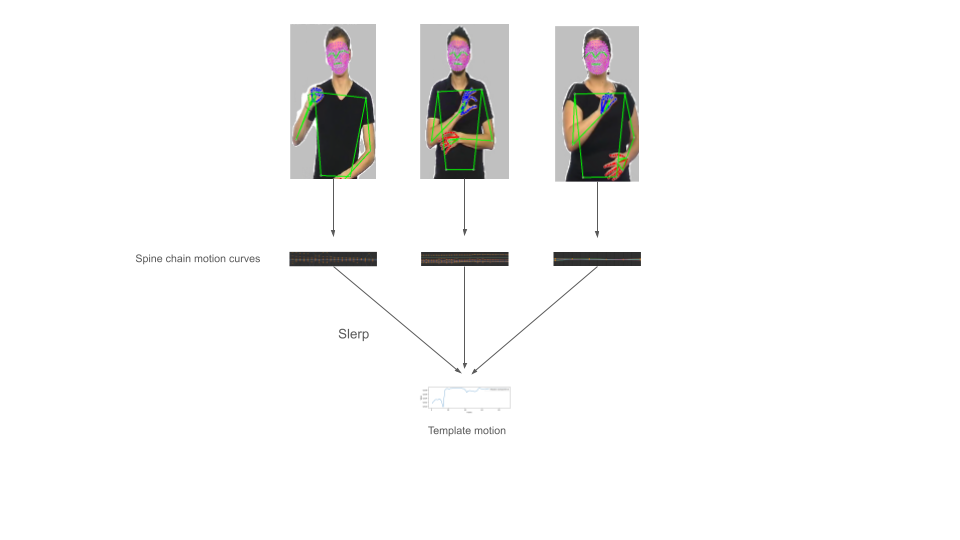
\includegraphics[width = 4in]{chapters/intermediate_blocks/images/motion_curves_template_procedural.png}
    \caption{Procedurally Generated motion curves for template \emph{info-about}}
    \label{fig:motion_curves_template_procedural}
\end{figure}

The template was created by extracting bone rotations as quaternions using mediapipe pose estimation and then converting them into motion curves (figure~\ref{fig:motion_curves_mediapipe}). The final blended rotation can be calculated using Spherical Linear Interpolation (Slerp) between \( n \) quaternions \( q_1, q_2, \dots, q_n \):

\[
q_{\text{blend}} = \text{Slerp}\left(\dots \text{Slerp}\left(\text{Slerp}(q_1, q_2, t_1), q_3, t_2 \right) \dots , q_n, t_{n-1} \right)
\]

Where:
\begin{itemize}
    \item \( t_1, t_2, \dots, t_{n-1} \) are the blend factors for each interpolation step, with \( t_i \in [0, 1] \).
    \item The Slerp between two quaternions \( q_i \) and \( q_j \) is defined as:
    \[
    \text{Slerp}(q_i, q_j, t) = \frac{\sin((1-t)\theta)}{\sin(\theta)} q_i + \frac{\sin(t\theta)}{\sin(\theta)} q_j
    \]
    where \( \theta = \arccos(q_i \cdot q_j) \) is the angle between the quaternions.
\end{itemize}

\begin{figure}
    \centering 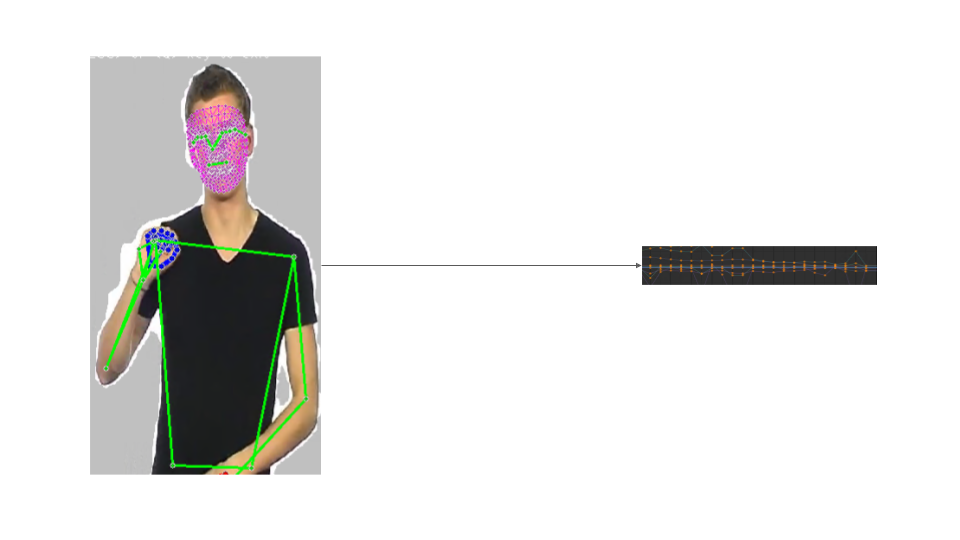
\includegraphics[width = 2.5in]{chapters/intermediate_blocks/images/motion_curves_mediapipe.png}
    \caption{Motion Curves from Mediapipe Pose Estimation}
    \label{fig:motion_curves_mediapipe}
\end{figure}

Figure~\ref{fig:motion_curves_mocap} similar template creation but using AZee annotated motion capture~\cite{bertin2022rosetta}.

\begin{figure}
    \centering 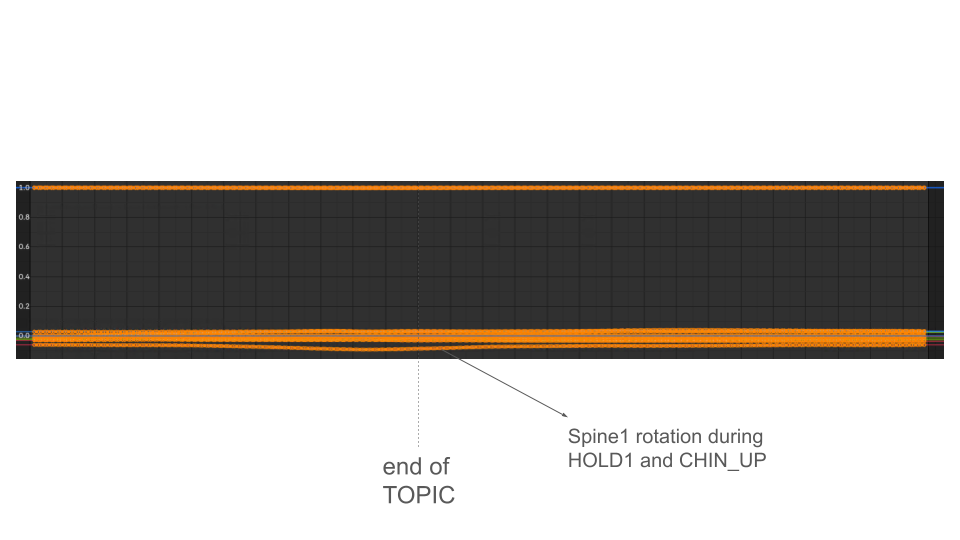
\includegraphics[width = 4in]{chapters/intermediate_blocks/images/motion_curves_mocap.png}
    \caption{Motion Curves from AZee annotated Mocap for the chin up in }
    \label{fig:motion_curves_mocap}
\end{figure}

Lastly, artistically created template for the rule \emph{about-ref} can be seen in the following figure~\ref{fig:motion_curves_template_artist}.

\begin{figure}
     \centering
    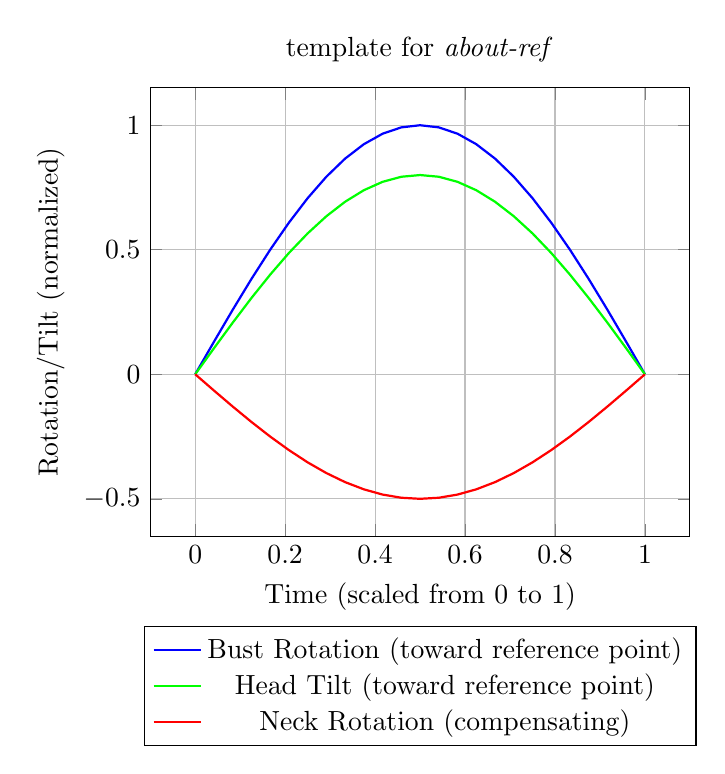
\begin{tikzpicture}
        \begin{axis}[
            title={template for \emph{about-ref}},
            xlabel={Time (scaled from 0 to 1)},
            ylabel={Rotation/Tilt (normalized)},
            grid=major,
            legend style={at={(0.5,-0.2)},anchor=north,legend columns=1} % Legend in two rows
        ]
        % Bust rotation
        \addplot[blue, thick, domain=0:1] {sin(deg(pi*x))};
        \addlegendentry{Bust Rotation (toward reference point)}
        
        % Head tilt
        \addplot[green, thick, domain=0:1] {0.8*sin(deg(pi*x))};
        \addlegendentry{Head Tilt (toward reference point)}
        
        % Neck rotation (compensating)
        \addplot[red, thick, domain=0:1] {-0.5*sin(deg(pi*x))};
        \addlegendentry{Neck Rotation (compensating)}
        
        \end{axis}
    \end{tikzpicture}
    \caption{Artistically Created motion curves for template \emph{about-ref}}
    \label{fig:motion_curves_template_artist}
\end{figure}

\section{Motion Curves}
\label{ch:intermediate_blocks:curves}

Motion curves are a fundamental component of character animation, providing a graphical representation of how a character's movements change over time. By manipulating these curves, animators can control the timing and spacing of movements, ensuring that the animation is realistic and expressive.

\subsection{Skeletal Motion Curves}
\label{ch:intermediate_blocks:curves:skeletal}

The template expression check determines the motion template to be used, which in turn gives us information regarding how a pair of blocks can be connected. However, these motion curves can either effect the skeleton, or the shape keys. For skeleton, these motion curves represent time in x axis, and the joint angle(FK) of the y axis. Each bone has has 4 motion curves (one for each axis of the quaternion rotation).

Figure~\ref{fig:motion_curves_skeletal} shows how motion curves can be used for skeleton for the above example.

\begin{figure}
    \centering 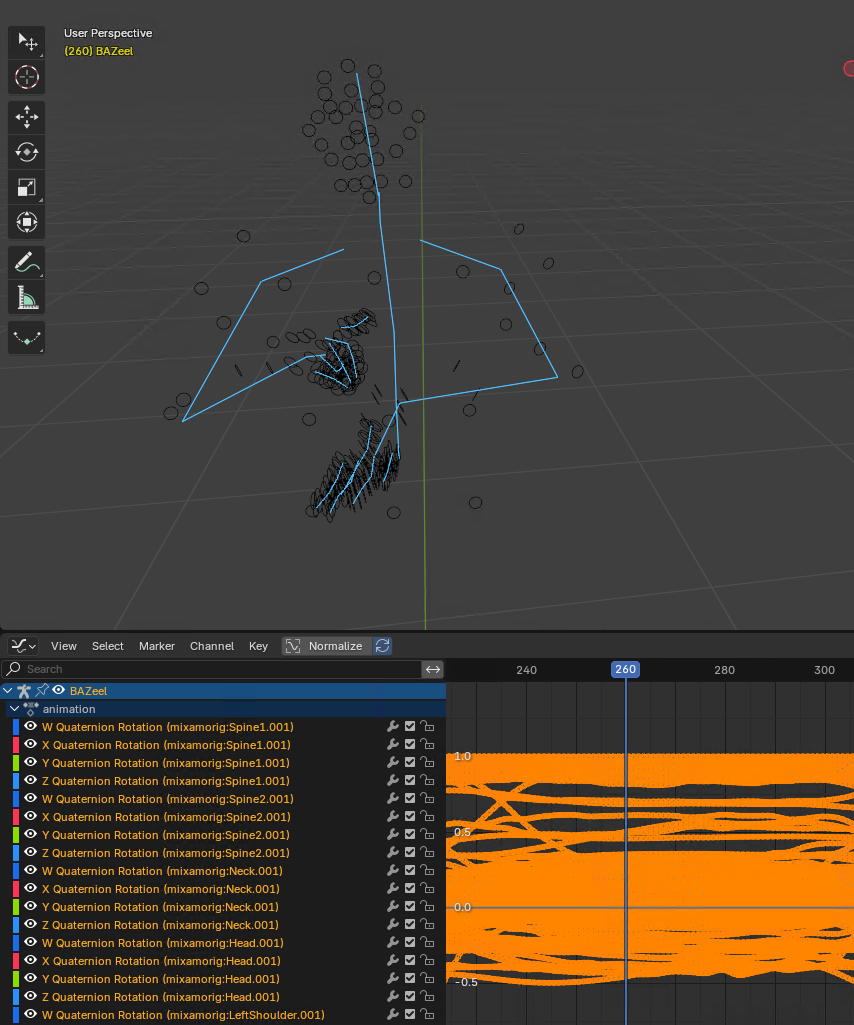
\includegraphics[width = 2.5in]{chapters/intermediate_blocks/images/motion_curves_skeletal.png}
    \caption{Motion Curves for Skeleton}
    \label{fig:motion_curves_skeletal}
\end{figure}

\subsection{Shape Key Motion Curves}
\label{ch:intermediate_blocks:curves:shape_keys}

For shape keys, the motion curves represent time in x axis, and the weight of the shape key in the y axis. Each shape key has one motion curve. Figure~\ref{fig:motion_curves_shape_keys} shows how motion curves can be used for shape keys for the facial expressions of the above example.

\begin{figure}
    \centering 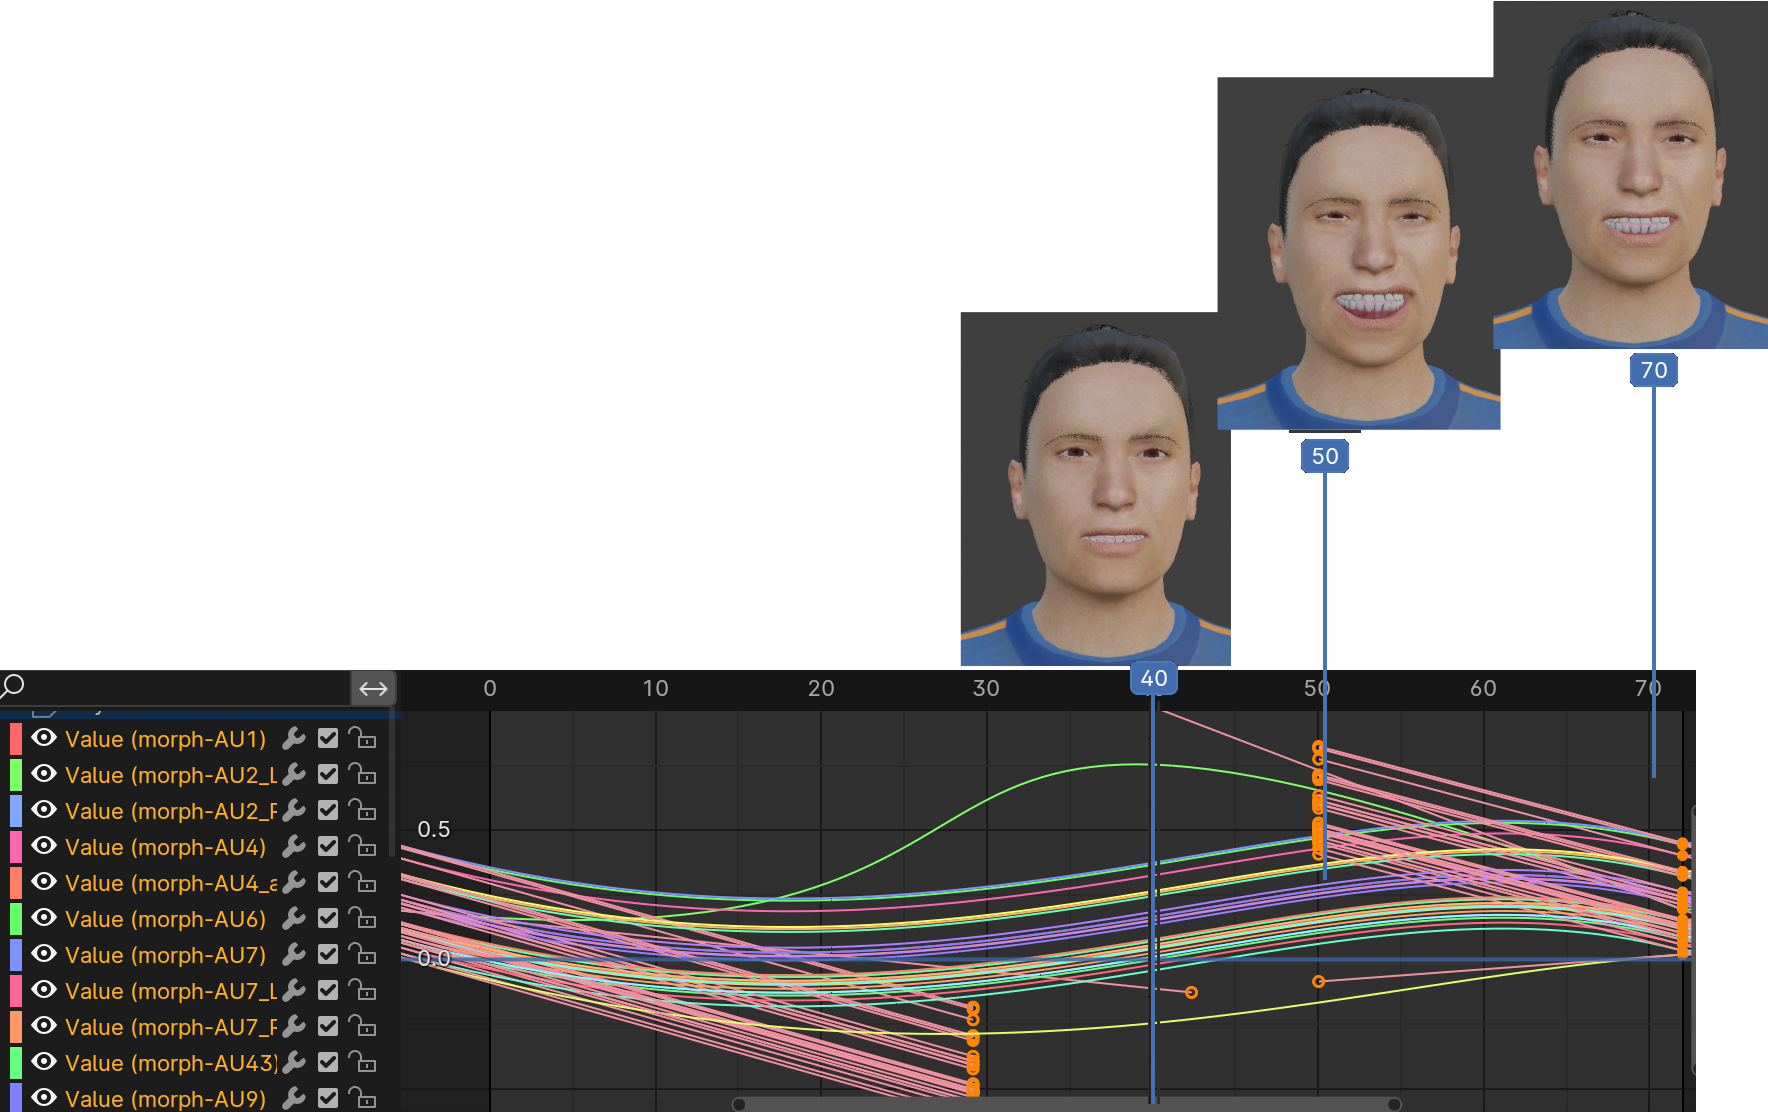
\includegraphics[width = 2.5in]{chapters/intermediate_blocks/images/motion_curves_shape_keys.png}
    \caption{Motion Curves for Shape Keys}
    \label{fig:motion_curves_shape_keys}
\end{figure}

\section{Results}
\label{ch:intermediate_blocks:results}

Figure~\ref{fig:intermediate_blocks_results} shows the results of the intermediate block generation process. The top row shows the original AZee blocks, while the bottom row shows the intermediate blocks generated using motion curves and templates. Motion curve comparison betweeen standard interpolation and interpolation based on the template for some AZee rules is shown in figure~\ref{fig:intermediate_blocks_comparison}.

\begin{figure}
    \centering \includegraphics[width = 2.5in]{chapters/intermediate_blocks/images/intermediate_blocks_results.png}
    \caption{Intermediate Block Generation Results}
    \label{fig:intermediate_blocks_results}
\end{figure}

\begin{figure}
    \centering \includegraphics[width = 2.5in]{chapters/intermediate_blocks/images/intermediate_blocks_comparison.png}
    \caption{Comparison with normal interpolation}
    \label{fig:intermediate_blocks_comparison}
\end{figure}

The complete animations can be seen in the following video: \url{todo}

An increase in naturalness when animating using the intermediate blocks technique can be seen. Moreover, this work provides us isnights regarding the motion profile which an AZee rul asbtracts.

\section{Conclusion and Future Work}
\label{ch:intermediate_blocks:conclusion_and_future_work}

In this chapter, we explored the generation of intermediate blocks in multi-track representations using motion curves and templates. By leveraging the AZee model and motion curves, we were able to create smooth transitions between constrained blocks, enhancing the naturalness and coherence of Sign Language synthesis. The results demonstrate the effectiveness of this approach compared to using standard block interpolation. 

%limitations
While the current system of motion templates proves effective for generating smooth transitions in most body movements, it faces significant challenges when dealing with finer details such as finger articulation. The complexity of finger movements in sign language, especially during rapid transitions, requires high precision in motion curves and templates. Unfortunately, the current implementation lacks the necessary granularity to handle the intricate dynamics of handshapes and finger configurations, often resulting in unnatural or robotic animations in these areas. Moreover, capturing the nuances of coarticulation between handshapes and other body parts remains an open challenge.

Another limitation stems from too much data in the motion templates. This might bring in information such as the identity of the signer, which may not always generalize well. While procedurally generated templates based on AZee rules offer flexibility, their 

Future areas to improve this technique could include a more detailed quantitative analysis of motion capture data based on a broader range of AZee rules, as well as further refinement of finger tracking and facial expressions in the motion templates.

Future areas to improve this technique could be a deeper quantitative analysis of mocap data based on more AZee rules. This could help in procedurally creating a more robust set of motion templates that can be used across different signing scenarios.

\end{document}